\documentclass[aspectratio=169,11pt]{beamer}

\usepackage{graphicx}
\usepackage{tikz}
\usetikzlibrary{positioning,arrows.meta}
\usepackage{xcolor}
\usepackage{booktabs}
\usepackage{tabularx}
\usepackage{array}
\usepackage{ragged2e}

\definecolor{GEUBlue}{RGB}{20,55,105}
\definecolor{GEULightBlue}{RGB}{238,244,251}
\definecolor{GEUGrey}{RGB}{90,90,90}
\definecolor{GEULightGrey}{RGB}{245,246,248}

\usetheme{default}
\setbeamertemplate{navigation symbols}{}
\setbeamertemplate{blocks}[rounded][shadow=false]
\setbeamercolor{normal text}{fg=black,bg=white}
\setbeamercolor{frametitle}{fg=GEUBlue}
\setbeamercolor{structure}{fg=GEUBlue}
\setbeamercolor{block title}{fg=GEUBlue,bg=GEULightBlue}
\setbeamercolor{block body}{fg=black,bg=GEULightBlue}
\setbeamerfont{frametitle}{size=\Large,series=\bfseries}

% Replace with the actual logo filename
\newcommand{\GEULogo}{graphicera_logo.png}

% Header and footer
\setbeamertemplate{headline}{%
  \begin{tikzpicture}[remember picture,overlay]
    \node[anchor=north east,xshift=-0.30cm,yshift=-0.12cm]
      at (current page.north east)
      {\includegraphics[height=0.62cm]{\GEULogo}};
  \end{tikzpicture}
  \vspace{0.72cm}
}
\setbeamertemplate{frametitle}{%
  \vspace{0.03cm}
  \insertframetitle\par
  \vspace{0.04cm}
  \textcolor{GEUBlue}{\rule{\textwidth}{0.9pt}}
  \vspace{0.03cm}
}
\setbeamertemplate{footline}{%
  \leavevmode
  \hbox{%
  \begin{beamercolorbox}[wd=.82\paperwidth,ht=0.32cm,dp=0.10cm,leftskip=.3cm]{author in head/foot}
    \tiny Department of Computer Science \& Engineering | Graphic Era (Deemed to be University)
  \end{beamercolorbox}%
  \begin{beamercolorbox}[wd=.18\paperwidth,ht=0.32cm,dp=0.10cm,rightskip=.3cm]{date in head/foot}
    \hfill\tiny\insertframenumber/\inserttotalframenumber
  \end{beamercolorbox}}
}

\newcommand{\smallnote}[1]{\vspace{0.08cm}{\scriptsize\color{GEUGrey}#1}}
\newcommand{\placeholder}[1]{\textit{\color{GEUGrey}#1}}

\title{\textbf{Project-Based Learning}\\[2mm]\large Phase-I Evaluation}
\author{\textbf{Project Title}\\Team ID: XXXX}
\institute{Department of Computer Science \& Engineering\\Graphic Era (Deemed to be University), Dehradun}
\date{Academic Session 2026--27}

\begin{document}

% 1
\begin{frame}[plain]
\begin{tikzpicture}[remember picture,overlay]
\draw[GEUBlue,line width=3pt] (current page.north west) -- (current page.north east);
\node[anchor=north east,xshift=-0.45cm,yshift=-0.35cm] at (current page.north east)
{\includegraphics[height=1.0cm]{\GEULogo}};
\node[align=center,text width=.84\paperwidth] at ([yshift=.25cm]current page.center)
{{\color{GEUBlue}\fontsize{26}{30}\selectfont\bfseries PROJECT-BASED LEARNING}\\[3mm]
 {\fontsize{18}{22}\selectfont PHASE-I EVALUATION}\\[7mm]
 {\color{GEUGrey}\Large\bfseries \placeholder{Automated Timetable Clash Detector and Resolver}}\\[3mm]
 {\color{GEUBlue}\normalsize Team ID: DSCPP-III-2026-T019}};
\node[align=center,anchor=south,yshift=.42cm] at (current page.south)
{\bfseries Department of Computer Science \& Engineering\\
Graphic Era (Deemed to be University), Dehradun\\[-1mm]
\scriptsize Academic Session 2026--27};
\end{tikzpicture}
\end{frame}

% 2
\begin{frame}{Team \& Mentor Details}
\begin{columns}[T,totalwidth=\textwidth]
\column{.48\textwidth}
\begin{block}{Team Information}
\begin{tabular}{@{}ll@{}}
\textbf{Team ID:} & DSCPP-III-2026-T019\\
\textbf{Semester:} & 3rd \\
\textbf{Section:} & A, C, E, G\\
\textbf{Domain:} & CSE\end{tabular}
\end{block}
\column{.48\textwidth}
\begin{block}{Team Members}
1.\quad \placeholder{Krish Singh Pujara -- 2510010141
}\\
2.\quad \placeholder{Kanak Bhatt -- 2510011122}\\
3.\quad \placeholder{Sanchit Gupta -- 2510010543
}\\
4.\quad \placeholder{Sara Raturi -- 2510012612
}
\end{block}
\end{columns}
\vspace{2mm}
\begin{block}{Mentor}
\placeholder{Ms. Megha Garg}
\hfill
\textbf{Interactions completed:} \underline{\hspace{12mm}2}
\end{block}
\end{frame}

% 3
\begin{frame}{Problem Statement \& Motivation}
\begin{block}{Problem Statement}
\placeholder{Colleges struggle with manual, error-prone timetable scheduling, leading to room, faculty, and section overlaps. Existing software often flags these conflicts but leaves staff to resolve them manually without explaining the underlying logic. This project addresses this gap by developing an automated C++ system that uses graph algorithms to actively detect, model, and resolve scheduling clashes without human intervention.}
\end{block}
\vspace{2mm}
\begin{columns}[T,totalwidth=\textwidth]
\column{.48\textwidth}
\textbf{\color{GEUBlue}Motivation}
\begin{itemize}\itemsep2pt
\item \placeholder{Manual scheduling, missing auto-fix.}
\item \placeholder{Disrupted academic schedules.}
\item \placeholder{Passive flagging, opaque logic.}
\end{itemize}
\column{.48\textwidth}
\textbf{\color{GEUBlue}Target Users / Stakeholders}
\begin{itemize}\itemsep2pt
\item \placeholder{College administrators.}
\item \placeholder{Students, faculty and institutional management.}
\item \placeholder{Automated clash-free scheduling.}
\end{itemize}
\end{columns}
\end{frame}

% 4
\begin{frame}{Objectives}
\textbf{\color{GEUBlue}Project Objectives}
\vspace{2mm}
\begin{enumerate}\itemsep5pt
\item \placeholder{Develop an automated timetable scheduling system.}
\item \placeholder{Implement sweep-line clash detection and resolution.}
\item \placeholder{Apply DSA and OOPS concepts in C++.}
\item \placeholder{Test algorithm performance and system correctness.}
\item \placeholder{Provide efficient and clash-free timetable output.}
\end{enumerate}
\vfill
\begin{center}
\colorbox{GEULightBlue}{\parbox{.80\textwidth}{\centering
\textbf{Key Objective:} \placeholder{To enable fast, efficient, and automated resolution of college timetable clashes.}}}
\end{center}
\end{frame}

% 5
\begin{frame}{Proposed Solution}
\begin{columns}[T,totalwidth=\textwidth]
\column{.48\textwidth}
\textbf{\color{GEUBlue}Proposed Approach}
\begin{enumerate}\itemsep3pt
\item \placeholder{Add Timetable Data}
\item \placeholder{Apply DSA Algorithms}
\item \placeholder{Resolve Scheduling Clashes}
\item \placeholder{Store Availability Records}
\item \placeholder{Display Conflict-Free Output}
\end{enumerate}
\column{.48\textwidth}
\textbf{\color{GEUBlue}Key Features}
\begin{itemize}\itemsep3pt
\item \placeholder{Detect Schedule Clashes}
\item \placeholder{Auto-Resolve Conflicts}
\item \placeholder{\textit{Fast Hash Lookup}}
\item \placeholder{Priority-Based Allocation}
\item \placeholder{View Resolved Timetable}
\end{itemize}
\end{columns}
\vfill
\smallnote{}
\end{frame}

% 6
\begin{frame}{Integration of PBL Course Concepts}
\scriptsize
\begin{center}
\renewcommand{\arraystretch}{1.25}
\begin{tabularx}{.96\textwidth}{@{}>{\bfseries}p{3.0cm}X p{2.5cm}@{}}
\toprule
Course & Concepts Applied & Project Module\\
\midrule
Data Structures in C & \placeholder{Arrays, Hash Tables, Graphs (DFS/BFS), Sorting} & \placeholder{Clash Detection \& Conflict Modeling}\\\\
\midrule
OOPs with C++ & \placeholder{Classes, Objects, Structures, STL Vectors} & \placeholder{Data Modeling \& Auto-Resolution Engine}\\

\bottomrule
\end{tabularx}
\end{center}
\vfill
\begin{center}
\end{center}
\end{frame}

% 7
\begin{frame}{System Architecture / Workflow}
\begin{center}
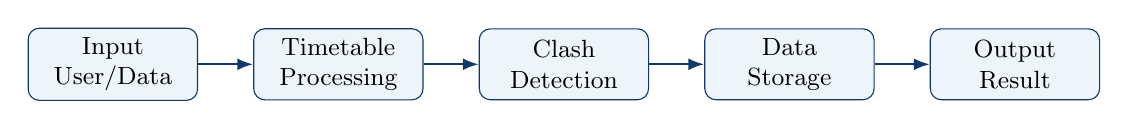
\begin{tikzpicture}[
node distance=7mm,
box/.style={rectangle,rounded corners,draw=GEUBlue,fill=GEULightBlue,
minimum width=2.15cm,minimum height=9mm,align=center,font=\small},
arrow/.style={-{Latex[length=2mm]},thick,draw=GEUBlue}
]
\node[box] (a) {Input\\User/Data};
\node[box,right=of a] (b) {Timetable\\Processing};
\node[box,right=of b] (c) {Clash\\Detection};
\node[box,right=of c] (d) {Data\\Storage};
\node[box,right=of d] (e) {Output\\Result};
\draw[arrow] (a)--(b); \draw[arrow] (b)--(c); \draw[arrow] (c)--(d); \draw[arrow] (d)--(e);
\end{tikzpicture}
\end{center}
\vspace{5mm}
\begin{columns}[T,totalwidth=\textwidth]
\column{.48\textwidth}
\textbf{\color{GEUBlue}Major Components}
\begin{itemize}\itemsep2pt
\item \placeholder{Timetable Management}
\item \placeholder{Clash Detection \& Analysis}
\item \placeholder{Clash Resolution}
\end{itemize}
\column{.48\textwidth}
\textbf{\color{GEUBlue}Data / Control Flow}
\begin{itemize}\itemsep2pt
\item \placeholder{User enters timetable details}
\item \placeholder{System checks teacher, room & section conflicts}
\item \placeholder{Available slots are identified and revised timetable is displayed}
\end{itemize}
\end{columns}
\end{frame}

% 8
\begin{frame}{Technology Stack \& Methodology}
\begin{columns}[T,totalwidth=\textwidth]
\column{.48\textwidth}
\begin{block}{Technology Stack}
\begin{itemize}\itemsep2pt
\item Programming: \placeholder{C++}
\item Database: \placeholder{PostgreSQL}
\item Tools / Framework: \placeholder{C++ STL}
\item IDE: \placeholder{VS Code}
\item Version Control: \placeholder{Git / GitHub}
\end{itemize}
\end{block}
\column{.48\textwidth}
\begin{block}{Development Methodology}
\begin{enumerate}\itemsep2pt
\item Requirement Analysis
\item System Design
\item Implementation
\item Testing
\item Evaluation
\end{enumerate}
\end{block}
\end{columns}
\vfill
\begin{center}
\end{center}
\end{frame}

% 9
\begin{frame}{Initial Progress \& Team Contribution}
\begin{columns}[T,totalwidth=\textwidth]
\column{.44\textwidth}
\textbf{\color{GEUBlue}Progress Achieved}
\begin{itemize}\itemsep3pt
\item \placeholder{Studied DSA concepts}
\item \placeholder{Identified core requirements}
\item \placeholder{Designed system architecture}
\item \placeholder{Implemented C++ models}
\item \placeholder{Prepared test datasets}
\end{itemize}
\column{.52\textwidth}
\textbf{\color{GEUBlue}Individual Contribution}
\vspace{2mm}
\scriptsize
\begin{tabularx}{\textwidth}{@{}p{1.8cm}p{2.0cm}X@{}}
\toprule
Member & Role & Contribution\\
\midrule
\placeholder{M1} & \placeholder{Lead} & \placeholder{System design}\\\\
\placeholder{M2} & \placeholder{Developer} & \placeholder{Core implementation}\\\\
\placeholder{M3} & \placeholder{DSA lead} & \placeholder{Clash Detection}\\\\
\placeholder{M4} & \placeholder{Developer/Docs} & \placeholder{Data modeling}\\
\bottomrule
\end{tabularx}
\end{columns}
\end{frame}

% 10
\begin{frame}{Roadmap, Expected Outcomes \& References}
\begin{columns}[T,totalwidth=\textwidth]
\column{.47\textwidth}
\textbf{\color{GEUBlue}Roadmap}
\begin{enumerate}\itemsep3pt
\item Phase-I: Proposal \& Design
\item Phase-II: Development
\item Phase-III: Final Implementation
\end{enumerate}
\vspace{2mm}
\textbf{\color{GEUBlue}Expected Outcomes}
\begin{itemize}\itemsep2pt
\item \placeholder{Working clash detection system}
\item \placeholder{Accurate conflict detection}
\item \placeholder{Clash resolution suggestions}
\item \placeholder{Efficient timetable management}
\end{itemize}
\column{.47\textwidth}
\textbf{\color{GEUBlue}References}
\begin{enumerate}\itemsep3pt
\item \placeholder{C++ Documentation}
\item \placeholder{DSA Textbook}
\item \placeholder{C++ STL Reference}
\item \placeholder{GitHub Repository}
\end{enumerate}
\vfill
\begin{center}
\colorbox{GEUBlue}{\parbox{.78\textwidth}{\centering\color{white}\textbf{Thank You}\\Questions \& Suggestions}}
\end{center}
\end{columns}
\end{frame}

\end{document}
